% !TEX encoding = UTF-8
% !TEX program = pdflatex
% !TEX spellcheck = it_IT

\documentclass[LaM,binding=0.6cm]{sapthesis}

\usepackage{microtype}
\usepackage[italian]{babel}
\usepackage[utf8]{inputenx}
\usepackage{booktabs}
\usepackage{tabularx}
\usepackage{graphicx}
\usepackage{dcolumn}
\usepackage{hyperref}
\usepackage{longtable}
\usepackage{pdflscape}
\usepackage{enumerate}
\hypersetup{pdftitle={Titolo della tesi},pdfauthor={Mario Greco}}

% Remove in a normal thesis
\usepackage{lipsum}
\usepackage{curve2e}
\definecolor{gray}{gray}{0.4}
\newcommand{\bs}{\textbackslash}

% Commands for the titlepage
\title{Titolo della tesi \\ bla bla bla}
\author{Mario Greco}
\IDnumber{984280}
\course{Informatica}
\courseorganizer{Facoltà di Ingegneria dell'Informazione, Informatica e Statistica}
\submitdate{2013/2014}
\copyyear{2014}
\advisor{Prof. Emanuele Panizzi}
% \advisor{Dr. Nome Cognome}
\coadvisor{Dott. Raffaele Gitto}
\authoremail{mrgreco3@gmail.com}

% \examdate{18 Marzo 2014}
% % \examiner{Prof. Nome Cognome}
% % \examiner{Prof. Nome Cognome}
% % \examiner{Dr. Nome Cognome}
\versiondate{\today}



\begin{document}

\frontmatter

\maketitle

\dedication{Dedicato a\\}

\begin{abstract}
.
\end{abstract}

\begin{acknowledgments}

\end{acknowledgments}

\tableofcontents

% % Do not use the starred version of the chapter command!
% \chapter{Capitolo non numerato}
% 
% In this manual you can skip the gray text because it is just dummy text.%
% \footnote{This is a footnote.}
% 
% \textcolor{gray}{\lipsum[1-22]}
% 
% 
% \section*{Paragrafo non numerato}
% 
% In this manual you can skip the gray text because it is just dummy text.
% 
% \textcolor{gray}{\lipsum[1-22]}




\mainmatter


\chapter{Introduzione al progetto}

\section{Descrizione dell'applicazione}



\section{Primi requisiti funzionali}
Di seguito sono riportati i primi requisiti funzionali ricavati dal processo di analisi delle richieste del committente, ottenute durante le interviste iniziali del progetto. Tali requisiti definiscono le funzionalità e i servizi 
offerti dal sistema da realizzare.

\begin{center}
       \captionof{table}{Primi requisiti funzionali}

    \begin{tabular}{p{6cm}|p{8cm}}

    \toprule
    \multicolumn{1}{c}{\textbf{Requisito funzionale}} &
    \textbf{Descrizione}\\

    \midrule
    Login ai servizi & Permettere all'utente l'accesso ai servizi bancari mediante credenziali \\
    Visualizzazione riepilogo conti e carte & Fornire opportune viste di riepilogo dei prodotti posseduti da un utente (esempio: conti correnti, carte di credito, ecc\dots)\\
    Visualizzazione storico saldi & Rappresentare tramite grafici dello storico saldi di un prodotto\\
    Riepilogo lista movimenti & Recuperare e visualizzare la lista dei movimenti di un determinato prodotto\\
    Filtraggio lista movimenti & Permettere il recupero dei movimenti in base un certo arco temporale\\
    Disporre operazioni bancarie & Permettere l'esecuzione di dispositive bancarie (esempio: bonifici, giroconti, ecc\dots) \\
    Interazione con i social network & Consentire la visualizzazione dei contenuti social messi a disposizione del cliente\\
    Messaggistica & Permettere la lettura delle comunicazioni ricevute  \\
    \bottomrule

    \end{tabular}
        \label{tab:requisiti_iniziali}

\end{center}



\section{Primi mockup, wireframe e prototipi}
\subsection{Mockup}
La realizzazione di mockup grafici ha permesso di offrire al cliente una prima rappresentazione visiva dei requisiti funzionali iniziali. Di seguito sono riportate alcuni di questi mockup relativi allo stadio iniziale del progetto.

\begin{figure}[!htbp]
\centering
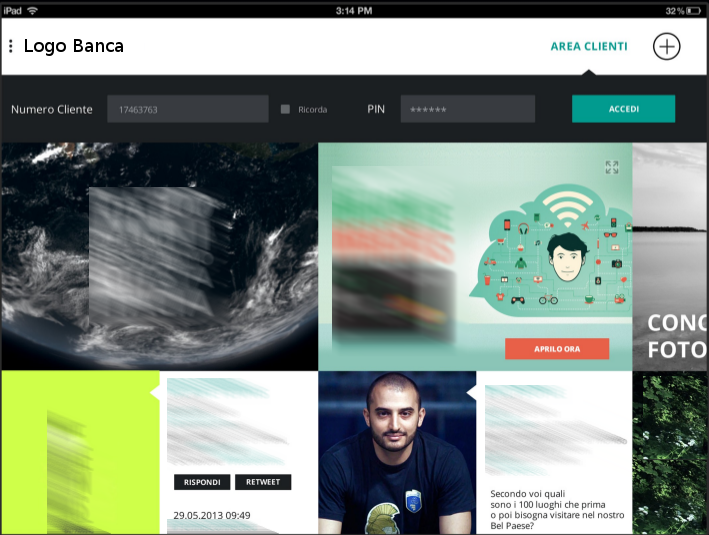
\includegraphics[scale=0.7]{immagini_mockup/home.png}
\caption{Home contenuti social e pannello login}
\end{figure}

\begin{figure}[!htbp]
\centering
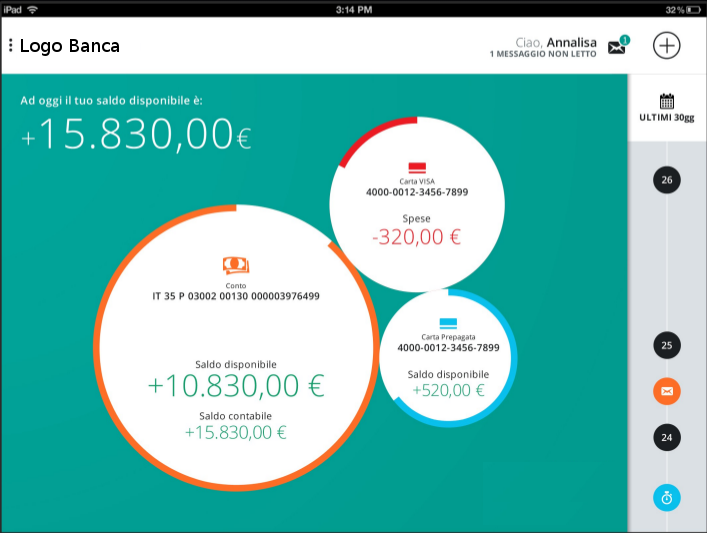
\includegraphics[scale=0.7]{immagini_mockup/bolle.png}
\caption{Riepilogo conti e carte}
\end{figure}

\begin{figure}[!htbp]
\centering
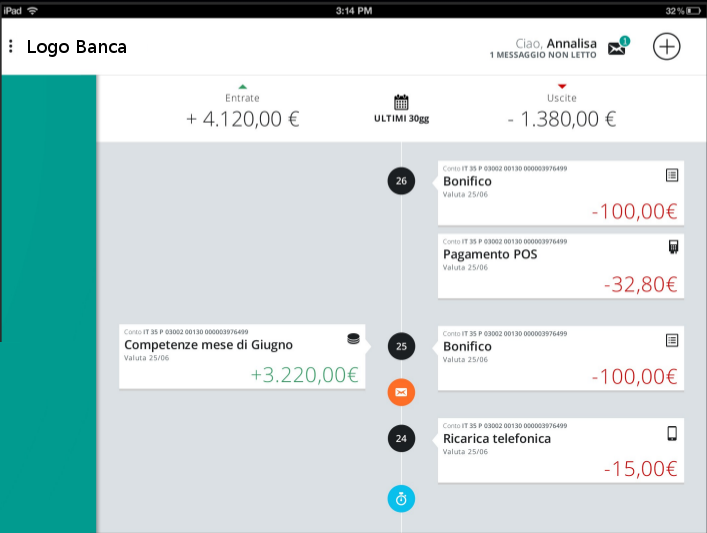
\includegraphics[scale=0.7]{immagini_mockup/timeline.png}
\caption{Timeline movimenti}
\end{figure}

\begin{figure}[!h]
\centering
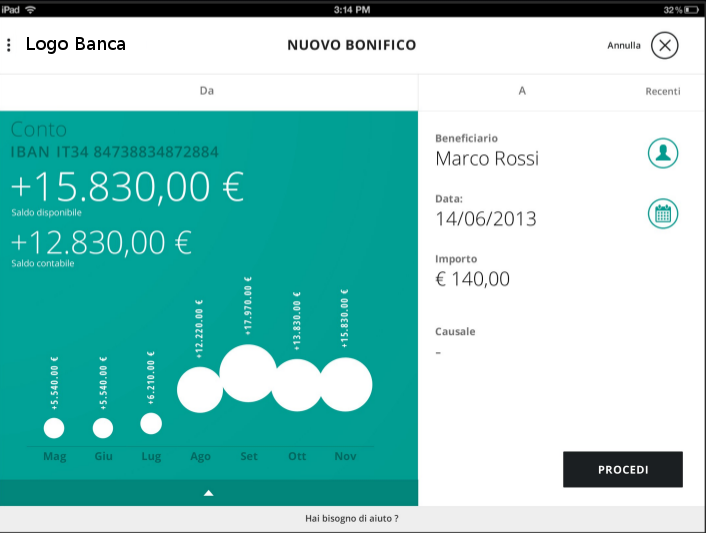
\includegraphics[scale=0.7]{immagini_mockup/bonifico.png}
\caption{Operazione bonifico}
\end{figure}

\newpage
\subsection{Wireframe}
Parallelamente ai mockup e durante tutto il ciclo di vita del software sono stati realizzati e raffinati i wireframe. 

I wareframe forniscono una rappresentazione strutturale di un applicazione software e permettono di individuare le dinamiche del progetto in termini di usabilità ed utilizzo pratico, i punti critici e quelli che richiedono uno sviluppo più accurato o miglioramenti.

Di seguito sono mostrate alcune delle immagini di uno dei primi wireframe realizzati:

\begin{figure}[!htbp]
\centering
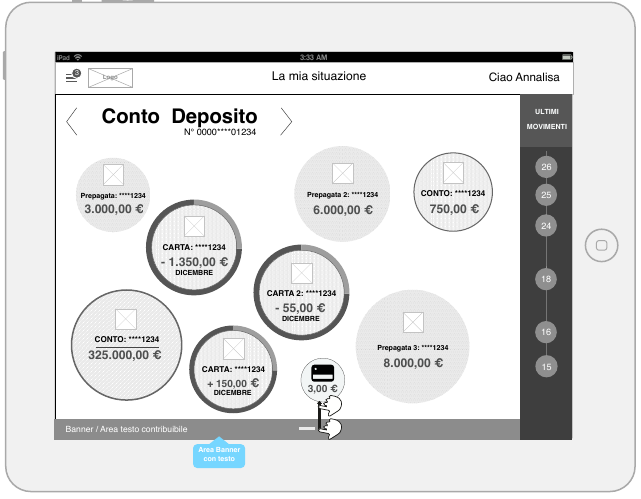
\includegraphics[scale=1.0]{primo_wireframe/miasituazione.png}
\caption{Riepilogo conti e carte}
\end{figure}
\begin{figure}[!htpb]
\centering
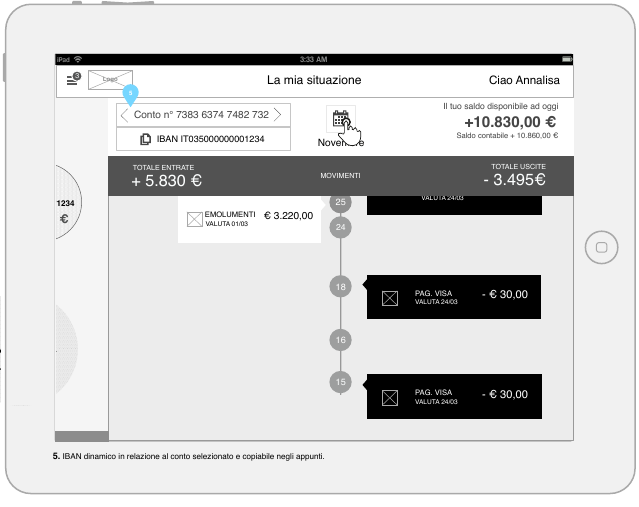
\includegraphics[scale=1.0]{primo_wireframe/timeline2.png}
\caption{Timeline movimenti}
\end{figure}
\begin{figure}[!htbp]
\centering
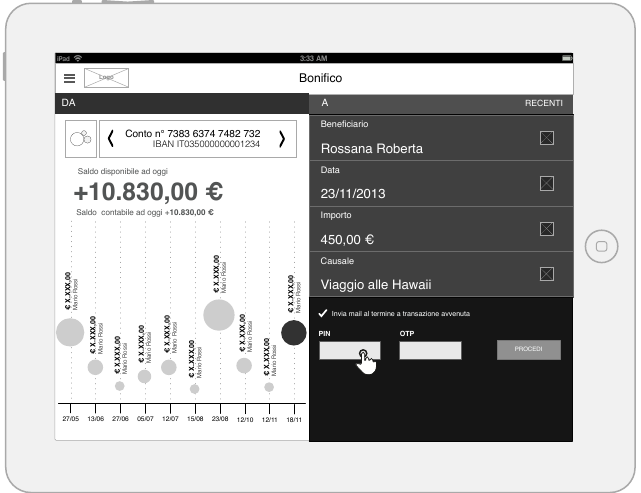
\includegraphics[scale=1.0]{primo_wireframe/bonifico2.png}
\caption{Dettaglio bonifico}
\end{figure}

\newpage
\subsection{Prototipi}
Un'altro passo fondamentale durante la fase iniziale del progetto è stato la realizzazione di prototipi.

Un prototipo è un modello approssimato del sistema che si sta realizzando e che simula o esegue solo una parte delle funzioni del sistema finale.
La prototipizzazione permette di:

\begin{itemize}
  \item tenere il design centrato sull’utente 
  \item sperimentare design alternativi
  \item ottenere feedback rapidi sul progetto
  \item trascurare dettagli secondari (come qualità del codice, efficienza, ecc\dots) 
  \item valutare l'usabilità
  \item ridurre i rischi di un progetto permettendoci di mettere prima a fuoco alcune caratteristiche del sistema e capire se sono adeguate o meno
\end{itemize}

Durante le prime settimane del progetto sono stati quindi realizzati dei prototipi contenenti funzionalità \emph{stub}\footnote{Funzionalità che simulano il comportamento  del sistema restituendo valori accettabili in un ipotetico scenario reale.} descritte dalla tabella \ref{tab:requisiti_iniziali}. Tali prototipi sono stati successivamente messi a disposizione del cliente e testati su device Apple iPad, portando alla raccolta e valutazione dei primi feedback sull'utilizzo del software.

\chapter{Metodologie usate e raffinamenti successivi}

\section{Metodologia Agile}

L'intero ciclo di vita del software è stato gestito adottando una metodologia \emph{Agile}.

I metodi Agile sono tali da coinvolgere il più possibile il committente, dando quindi vita a un processo di tipo adattativo: cioè che si adatta alle esigenze del cliente, che possono cambiare durante lo sviluppo.
L'Agile è un processo costituito da finestre di tempo limitate (2-4 settimane) chiamate iterazioni, le quali sono a loro volta scomposte nelle fasi di progettazione, di sviluppo e di test.

\begin{figure}[htbp]
\centering
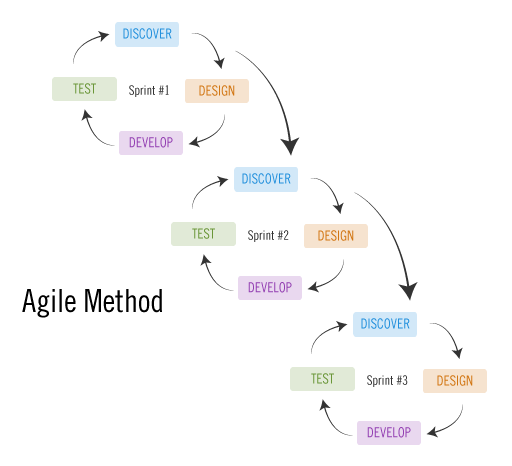
\includegraphics[scale=0.6]{immagini/agile.png}
\caption{Iterazioni e fasi della metodologia Agile}
\end{figure}

Il progetto è quindi suddiviso in singoli componenti indipendenti dalle funzionalità così da poterne analizzare e valutare i costi e i tempi. Ogni iterazione conterrà quindi tutto ciò che è indispensabile per rilasciare un piccolo incremento nelle funzionalità del software e sono tali da essere soggette a modifiche al fine di migliorare l'architettura finale del software.
% Anche se in un'iterazione non si hanno sufficienti funzionalità per ottenere un componente completo, esso deve esser rilasciato e nelle iterazioni successive dovrà avvicinarsi alle richieste del cliente.
% 
% Anche se il risultato di ogni singola
% iterazione non ha sufficienti funzionalità da essere considerato completo,
% deve essere rilasciato e nel susseguirsi delle iterazioni, deve avvicinarsi
% sempre di più alle richieste del cliente. Alla fine di ogni iterazione il team
% dovrà rivalutare le priorità del progetto.
% 
% Ogni iterazione è progetto a sé
% stante e deve contenere tutto ciò che è necessario per rilasciare un piccolo
% incremento nelle funzionalità del software: pianificazione (user stories),
% design, implementazione, test. An
% 
% Sulla scorta di queste considerazioni, nelle metodologie agili i vincoli principali dei progetti
% diventano i tempi, i costi e la possibilità di favorire la gestione del cambiamento dei requisiti.
% Naturalmente, per poter operare in tal modo, è richiesta la suddivisione in singoli componenti
% indipendenti delle funzionalità, al fine di poterne valutare i tempi, i costi e la possibilità di
% completarli procedendo per piccoli incrementi progressivi. In tal modo, viene agevolata anche la
% suddivisione dei compiti e delle responsabilità ai componenti del team di sviluppo.
% In definitiva, i Metodi Agili [21] sono un insieme di tecniche di sviluppo software che si
% focalizzano sullo sviluppo ed il rilascio incrementale (ed in tempi brevi) di porzioni del sistema, che
% siano usabili.
% 
% 
% 
% A differenza delle metodologie "pesanti", quelle agili sono caratterizzate da un processo
% iterativo scomposto in fase di progettazione, di sviluppo e test96 di breve durata.
% Tipicamente, i Metodi Agili si basano su di una disciplina rigorosa che dà vita ad un processo
% ben definito; si noti, però, che quest'ultimo è di tipo adattativo: si adatta, cioè, alle esigenze del
% committente, che possono mutare durante lo sviluppo. Quest'ultimo di focalizza su gruppi di
% funzionalità ed è guidato dalla necessità di rilasciare prodotti di progetto usabili.
% Dunque, gli artefatti possono considerarsi "leggeri", cioè manca la "pesante" documentazione.
% Il lavoro di progettazione, anzichè essere concentrato nella sola parte iniziale, è continuo e
% distribuito lungo tutte le fasi del processo. Pertanto, anche le parti già realizzate sono soggette a
% modifiche, al fine di migliorare l'architettura del software.
% 
% 
% Da ultima troviamo le metodologie agili. Questo particolare metodo di
% sviluppo software, a differenza dei precedenti, coinvolge quanto più
% possibile il committente, ottenendo in tal modo un elevata reattività alle
% sue richieste.
% La gran parte dei metodi agili tentano di ridurre il rischio di fallimento
% sviluppando il software in finestre di tempo limitate chiamate iterazioni
% che in genere durano qualche settimana. Ogni iterazione è progetto a sé
% stante e deve contenere tutto ciò che è necessario per rilasciare un piccolo
% incremento nelle funzionalità del software: pianificazione (user stories),
% design, implementazione, test. Anche se il risultato di ogni singola
% iterazione non ha sufficienti funzionalità da essere considerato completo,
% deve essere rilasciato e nel susseguirsi delle iterazioni, deve avvicinarsi
% sempre di più alle richieste del cliente. Alla fine di ogni iterazione il team
% dovrà rivalutare le priorità del progetto.
% 
% Un'importante constatazione che ha spinto verso questo approccio riguarda la natura mutevole
% nel tempo dei requisiti di un progetto. Pertanto, nell'ottica della pianificazione delle attività, i
% requisiti iniziali potrebbero risultare un punto di partenza inadeguato.
% L'adozione di un approccio è strettamente vincolato alla natura dei requisiti utente: del resto,
% sebbene averne cognizione definitiva già dal principio sia un aspetto desiderabile in qualunque
% progetto software, ciò avviene raramente. Inoltre, anche se accadesse, la fase di progettazione
% potrebbe ugualmente presentare qualche difficoltà.

\section{Requisiti funzionali finali}

Una progettazione iterativa e focalizzata sull'utente ha permesso quindi di ampliare e raffinare i requisiti fino ad ottenere  un risultato sempre più vicino alle richieste e alle necessità del committente.  

Per brevità di seguito sono riportati solo alcuni dei requisiti finali del progetto (che vanno ad aggiungersi o a integrare quelli della tabella \ref{tab:requisiti_iniziali}), per comodità racchiusi in categorie.
\begin{center}
   
    \begin{longtable}{p{6cm}|p{8cm}}

    \toprule
    \multicolumn{1}{c}{\textbf{Requisito funzionale}} &
    \textbf{Descrizione}\\

    \midrule
    Accesso ai servizi & \begin{itemize}
                          \item Permettere l'accesso ai servizi attraverso credenziali
                          \item Permette accesso veloce a un sottoinsieme di funzioni salvando le credenziali
                          \item Permettere recupero Codice Cliente
                         \end{itemize}\\

    Riepilogo movimenti & \begin{itemize}
                           \item Rappresentare i movimenti di un conto attraverso una timeline (timeline)
                           \item Mostrare i movimenti di un conto in una lista
                           \item Visualizzare una scheda di dettaglio per un movimento selezionato
                          \end{itemize}\\
    Filtro movimenti & Offrire la possibilità di filtrare i movimenti per data e per tipo (entrate, uscite, tutti)\\
    Riepilogo conti e carte & Visualizzare i prodotti di un utente mediante bubble contenenti informazioni di riepilogo\\
    Filtro conti e carte & Permettere la visualizzazione o meno di certi prodotti mediante un filtro\\
    Storico saldi & Visualizzare in un grafico a bolle lo storico dei saldi per mesi o settimane di un prodotto\\
    Disporre operazioni bancarie & \begin{itemize}
				      \item Permettere l'esecuzione di dispositive
				      \item Permettere la riproposizione di dispositive già effettuate
				    \end{itemize}\\
    Riepilogo dispositive effettuate & \begin{itemize}
                                        \item Visualizzare le ultime n dispositive in una lista ordinata
                                        \item Visualizzare le ultime n dispositive in un grafico a bolle
                                        \item Permettere il salvataggio delle dispositive effettuate in una lista di preferiti
                                       \end{itemize}\\
    Preferiti & Permettere la visualizzazione e la modifica di una lista di dispositive scelte come preferite\\
    Rubrica & Permettere l'accesso in lettura e scrittura alla rubrica del dispositivo per poter salvare o recuperare numeri telefonici\\
    
    Help e gestore & \begin{itemize}
                      \item Offrire una sezione interna al software in cui l'utente può richiedere appuntamenti con un consulente
                      \item Mettere a disposizione una sezione di help e numeri utili
                     \end{itemize}\\

    Integrazione social network & \begin{itemize}
                                   \item Visualizzare i contenuti dei canali social offerti dal committente
                                   \item Offrire la possibilità di condividere i contenuti sui diversi social network
				   \item Integrare un player video per la visualizzazione di filmati relativi alle attività del committente
                                  \end{itemize}\\
     Browsing interno & Permettere la navigazione tra contenuti web attraverso un browser interno all'applicazione\\
     Notifiche Push & Permettere la ricezione di notifiche push\\
    
    \bottomrule

    \end{longtable}
    \captionof{table}{Requisiti funzionali finali}
\end{center}

Sono inoltre elencati alcuni dei requisiti non funzionali:

\begin{center}
   
    \begin{tabular}{p{6cm}|p{8cm}}

    \toprule
    \multicolumn{1}{c}{\textbf{Requisito non funzionale}} &
    \textbf{Descrizione}\\

    \midrule
    Comunicazione sicura & \begin{itemize}
                            \item Garantire la comunicazione sicura tra client e server
                            \item Garantire che i dati salvati all'interno del device siano protetti
                           \end{itemize}\\
    Ottimizzazione flusso dati & Limitare il più possibile il consumo dei dati\\
    Efficienza & Garantire uso efficiente delle risorse offerte dal device (cpu, batteria, ecc\dots)\\

    \bottomrule

    \end{tabular}
    \captionof{table}{Requisiti non funzionali}
        \label{tab:requisiti_non_funz}

\end{center}


\chapter{Casi d'suo}
I casi d'uso permettono di modellare il comportamento del sistema e descrivere i requisiti funzionali in linguaggio naturale. Grazie a questi modelli è quindi possibile rappresentare il comportamento esterno del sistema, visto come una black-box, dal punto di vista di un'attore.

Oltre a una descrizione testuale (gli \emph{Scenari}) i casi d'uso possono esser rappresentati mediante diagrammi. In tali diagrammi troviamo le segunti entità:
 \begin{itemize}
  \item gli attori: essi rappresentano un soggetto o un'entità esterna che interagisce col sistema
  \item i casi d'uso: rappresentano un particolare scenario di interazione tra attore e sistema. Sono rappresentati graficamente da ellissi
  \item le associazioni: rappresentate da una linea mettono in comunicazione un attore con i caso d'uso
 \end{itemize}

 Nei prossimi paragrafi saranno mostrati alcuni dei casi d'uso modellati durante la fase di analisi.
 \newpage
 
 \section{Diagrammi dei casi d'uso}
 
 \subsection{Caso d'uso: Ricarica telefonica}
	\begin{figure}[!htbp]
	  \centering
	  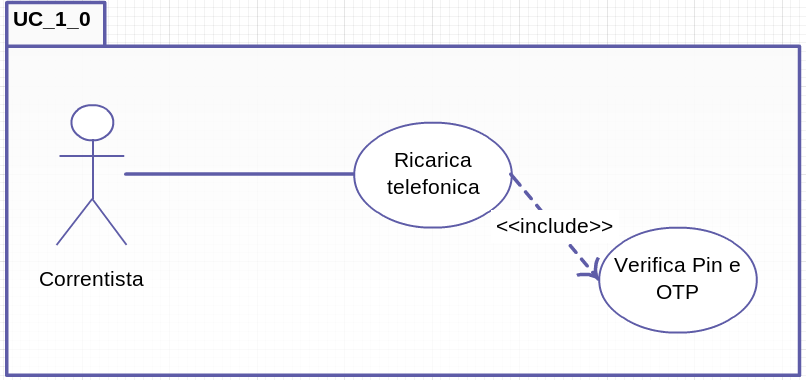
\includegraphics[scale=0.65]{casi_uso/ricarica.png}
	\end{figure}
	
  \subsection{Caso d'uso: Ricarica telefonica}
 	\begin{figure}[!htbp]
	  \centering
	  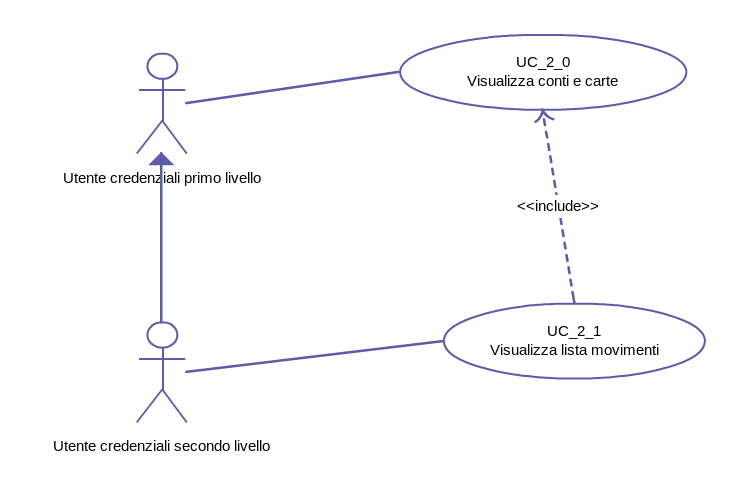
\includegraphics[scale=0.65]{casi_uso/conti.png}
	\end{figure}
	

 \section{Specifica dei casi d'uso}
 
 \subsection{Caso d'uso: Ricarica telefonica}

 Le tabelle \ref{tab:uc1}, \ref{tab:uc2}, \ref{tab:uc3}, \ref{tab:uc4}, \ref{tab:uc5} mostrano i casi d'uso relativi all'operazione di ricarica telefonica, nel caso in cui l'utente decida di ricaricare un numero di telefono associato ad un contatto presente nella rubrica del dispositivo.
 
 
\begin{center}
    \captionof{table}{Caso d'uso ricarica telefonica}
    \label{tab:uc1}
     \begin{longtable}{{ | l | p{8cm} |}}
    \hline
    \textbf{Caso d'uso} UC\_1\_0 & Ricarica telefonica di un numero salvato in rubrica \\ \hline
    \textbf{Attore} & Correntista bancario  \\ \hline
    \textbf{Precondizioni} & L'utente è loggato al sistema e ha iniziato una sessione inserendo un codice OTP  \\ \hline
    \textbf{Postcondizioni di successo}  & Il sistema ha registrato l'operazione \\\hline
    \textbf{Postcondizioni di fallimento}   &  Il sistema non ha registrato l'operazione\\\hline
    \textbf{Scenario} &  \\\hline
    & \begin{enumerate}
       \item L'utente seleziona l'operazione di ricarica telefonica \label{item:sel8}
       \item \texttt{Include} UC\_1\_1 \emph{Visualizza lista beneficiari}
       \item \texttt{Include} UC\_1\_2 \emph{Visualizza lista conti di addebito}
       \item \texttt{Include} UC\_1\_3 \emph{Visualizza lista operatori}
       \item \texttt{Include} UC\_1\_4 \emph{Verifica pin e OTP}
       
%        \item \label{item:sel1}Il sistema visualizza l'elenco dei beneficiari
%        \item L'utente seleziona un beneficiario 
%        \item \label{item:sel2}Il sistema visualizza l'elenco dei conti per l'addebbito
%        \item L'utente seleziona un conto
%        \item \label{item:sel3}\label{item:compagnia} Il sistema mostra l'elenco delle compagnie telefoniche
%        \item L'utente seleziona una compagnia telefonica
%        \item \label{item:sel4}Il sistema visualizza i tagli disponibili
%        \item L'utente seleziona un taglio di ricarica
%        \item \label{item:sel5}\label{item:beneficiario} Il sistema mostra il riepilogo dell'operazione e richiede conferma
%        \item L'utente conferma i dati
%        \item \label{item:credenziali}\label{item:sel6}Il sistema richiede Pin e OTP
%        \item L'utente immette i dati richiesti e conferma
%        \item \texttt{Include} \emph{Verifica credenziali}
       \item Il sistema mostra lo scontrino dell'operazione
      \end{enumerate}\\\hline
      \textbf{Scenari alternativi} &  \\\hline
     & \begin{itemize}
       \item  \ref{item:sel8} L'utente annulla operazione
       \item Il caso d'uso termina
      \end{itemize}\\\hline
     \end{longtable}
\end{center}

\begin{center}   
    \captionof{table}{Caso d'uso selezione beneficiario}
    \label{tab:uc2}
     \begin{longtable}{{ | l | p{8cm} |}}
    \hline
    \textbf{Caso d'uso} UC\_1\_1 & Selezione beneficiario \\ \hline
    \textbf{Attore} & Correntista bancario  \\ \hline
    \textbf{Precondizioni} & L'utente ha iniziato una nuova ricarica telefonica \\ \hline
    \textbf{Postcondizioni di successo}  & Il sistema ha convalidato la scelta del beneficiario \\\hline
    \textbf{Postcondizioni di fallimento}   &  Il sistema non ha cambiato stato\\\hline
    \textbf{Scenario} &  \\\hline
    & \begin{enumerate}
       \item \label{item:beneficiario} Il sistema visualizza la lista dei beneficiari
       \item L'utente seleziona un beneficiario 
       \item Il sistema aggiorna l'interfaccia con la selezione effettuata 
      \end{enumerate}\\\hline
      \textbf{Scenari alternativi} &  \\\hline
    & \begin{enumerate}
    \setcounter{enumi}{1}
       \item L'utente seleziona la voce \emph{Beneficiario}
       \item Il caso d'uso riprende dal punto \ref{item:beneficiario}
      \end{enumerate}\\\hline
     & \begin{itemize}
       \item L'utente annulla l'operazione
       \item Il caso d'uso termina
      \end{itemize}\\\hline

     \end{longtable}
\end{center}

\begin{center}
    \captionof{table}{Caso d'uso selezione conto di addebito}
    \label{tab:uc3}
     \begin{longtable}{{ | l | p{8cm} |}}
    \hline
    \textbf{Caso d'uso} UC\_1\_2 & Selezione conto di addebito \\ \hline
    \textbf{Attore} & Correntista bancario  \\ \hline
    \textbf{Precondizioni} & L'utente ha iniziato una nuova ricarica telefonica \\ \hline
    \textbf{Postcondizioni di successo}  & Il sistema ha convalidato la scelta del conto \\\hline
    \textbf{Postcondizioni di fallimento}   &  Il sistema non ha cambiato stato\\\hline
    \textbf{Scenario} &  \\\hline
    & \begin{enumerate}
       \item \label{item:conto} Il sistema visualizza la lista dei conti disponibili
       \item L'utente seleziona un conto 
       \item Il sistema aggiorna l'interfaccia con la selezione effettuata 
      \end{enumerate}\\\hline
      \textbf{Scenari alternativi} &  \\\hline
    & \begin{enumerate}
    \setcounter{enumi}{1}
       \item L'utente seleziona la voce \emph{Conto di addebito}
       \item Il caso d'uso riprende dal punto \ref{item:conto}
      \end{enumerate}\\\hline
     & \begin{itemize}
       \item L'utente annulla l'operazione
       \item Il caso d'uso termina
      \end{itemize}\\\hline
     \end{longtable}
\end{center}

\begin{center}
    \captionof{table}{Caso d'uso selezione operatore}
    \label{tab:uc4}
     \begin{longtable}{{ | l | p{8cm} |}}
    \hline
    \textbf{Caso d'uso} UC\_1\_3 & Selezione operatore \\ \hline
    \textbf{Attore} & Correntista bancario  \\ \hline
    \textbf{Precondizioni} & L'utente ha iniziato una nuova ricarica telefonica \\ \hline
    \textbf{Postcondizioni di successo}  & Il sistema ha convalidato la scelta dell'operatore \\\hline
    \textbf{Postcondizioni di fallimento}   &  Il sistema non ha cambiato stato\\\hline
    \textbf{Scenario} &  \\\hline
    & \begin{enumerate}
       \item \label{item:compagnia}Il sistema visualizza la lista delle compagnie telefoniche
       \item L'utente seleziona una compagnia 
       \item \label{item:tagli} Il sistema mostra i tagli di ricarica disponibili
       \item L'utente seleziona un taglio di ricarica
       \item Il sistema aggiorna l'interfaccia con la selezione effettuata
      \end{enumerate}\\\hline
      \textbf{Scenari alternativi} &  \\\hline
    & \begin{enumerate}
    \setcounter{enumi}{1}
       \item L'utente seleziona la voce \emph{Importo}
       \item Il caso d'uso riprende dal punto \ref{item:tagli}
      \end{enumerate}\\\hline
     & \begin{itemize}
       \item L'utente annulla l'operazione
       \item Il caso d'uso termina
      \end{itemize}\\\hline
    \textbf{Scenari di errore} &  \\\hline
    & \begin{enumerate}
    \setcounter{enumi}{1}
       \item L'utente seleziona una compagnia telefonica errata
       \item Il sistema mostra messaggio di errore
       \item Il caso d'uso riprende dal punto \ref{item:compagnia}
      \end{enumerate}\\\hline

     \end{longtable}
\end{center}

\begin{center}
    \captionof{table}{Caso d'uso verifica Pin e OTP}
    \label{tab:uc5}
     \begin{longtable}{{ | l | p{8cm} |}}
    \hline
    \textbf{Caso d'uso} UC\_1\_4 & Verifica Pin e OTP \\ \hline
    \textbf{Attore} & Correntista bancario  \\ \hline
    \textbf{Precondizioni} & L'utente ha iniziato una nuova ricarica telefonica e ha immesso tutti i dati richiesti\\ \hline
    \textbf{Postcondizioni di successo}  & Il sistema ha convalidato l'operazione e ha aggiornato il suo stato \\\hline
    \textbf{Postcondizioni di fallimento}   &  Il sistema non ha convalidato l'operazione e ha mostrato un messaggio di errore\\\hline
    \textbf{Scenario} &  \\\hline
    & \begin{enumerate}
       \item  Il sistema mostra il riepilogo dell'operazione e richiede conferma
       \item L'utente conferma i dati
       \item \label{item:credenziali}Il sistema richiede Pin e OTP
       \item L'utente immette i dati richiesti e conferma
       \item Il sistema verifica le credenziali
       \item Il sistema mostra lo scontrino dell'operazione effettuata
     \end{enumerate}\\\hline
      \textbf{Scenari alternativi} &  \\\hline
     & \begin{itemize}
       \item L'utente annulla l'operazione
       \item Il caso d'uso termina
      \end{itemize}\\\hline
     & \begin{enumerate}
      \setcounter{enumi}{4}
       \item Il sistema non valida le credenziali
       \item Il sistema visualizza tipo il di errore
       \item Il caso d'uso riprende dal punto \ref{item:credenziali}
      \end{enumerate}\\\hline
     \end{longtable}
\end{center}

 \subsection{Caso d'uso: Visualizza lista conti e carte e Visualizza lista movimenti}

\begin{center}
    \captionof{table}{Caso d'uso visualizza conti e carte}
    \label{tab:uc6}
     \begin{longtable}{{ | l | p{8cm} |}}
    \hline
    \textbf{Caso d'uso} & UC\_2\_0  Visualizza lista conti e carte \\ \hline
    \textbf{Attore} & Correntista bancario  \\ \hline
    \textbf{Precondizioni} & L'utente ha effettuato un login di primo o secondo livello \\ \hline
    \textbf{Postcondizioni di successo}  & Il sistema rimane nel suo stato o aggiorna la lista dei conti in memoria \\\hline
    \textbf{Postcondizioni di fallimento}   &  Il sistema rimane nel suo stato\\\hline
    \textbf{Scenario} &  \\\hline
    & \begin{enumerate}
       \item L'utente seleziona l'operazione di visualizzazione lista conti e carte
       \item \label{item:verificalista}Il sistema verifica che l'elenco dei prodotti non è vuoto
       \item Il sistema mostra la lista dei prodotti
      \end{enumerate}\\\hline
    \textbf{Scenario alternativo} &  \\\hline
    & \begin{enumerate}
    \setcounter{enumi}{1}
       \item Il sistema ha verificato che la lista dei prodotti è vuota
       \item Il sistema notifica l'evento con un opportuno messaggio
	\item Il caso d'uso termina
       \end{enumerate}\\\hline
    \textbf{Scenario di errore} &  \\\hline
    & \begin{enumerate}
    \setcounter{enumi}{1}
       \item Il sistema riceve un errore
       \item Il sistema notifica l'evento con un messaggio di errore e la possibilità di riprovare l'azione
       \item L'utente seleziona \emph{riprova}
       \item Il caso d'uso riprende dal punto \ref{item:verificalista}
       \end{enumerate}\\\hline
     \end{longtable}
\end{center}

\begin{center}
    \captionof{table}{Caso d'uso visualizza lista movimenti}
    \label{tab:uc7}
     \begin{longtable}{{ | l | p{8cm} |}}
    \hline
    \textbf{Caso d'uso} & UC\_2\_1  Visualizza lista movimenti \\ \hline
    \textbf{Attore} & Correntista bancario  \\ \hline
    \textbf{Precondizioni} & L'utente ha effettuato un login di secondo livello \\ \hline
    \textbf{Postcondizioni di successo}  & Il sistema rimane nel suo stato \\\hline
    \textbf{Postcondizioni di fallimento}   &  Il sistema rimane nel suo stato\\\hline
    \textbf{Scenario} &  \\\hline
    & \begin{enumerate}
       \item \texttt{Include} UC\_2\_0 \emph{Visualizza lista conti e carte}
       \item L'utente seleziona un conto o una carta
       \item \label{item:verificamovimenti}Il sistema verifica che la lista dei movimenti non è vuoto
       \item Il sistema mostra la lista dei prodotti
      \end{enumerate}\\\hline
    \textbf{Scenario alternativo} &  \\\hline
    & \begin{enumerate}
    \setcounter{enumi}{1}
       \item Il sistema ha verificato che la lista dei movimenti è vuota
       \item Il sistema notifica l'evento con un opportuno messaggio
	\item \texttt{Extend} \emph{Filtra movimenti per data}
       \end{enumerate}\\\hline
    \textbf{Scenario di errore} &  \\\hline
    & \begin{enumerate}
    \setcounter{enumi}{1}
       \item Il sistema riceve un errore
       \item Il sistema notifica l'evento con un messaggio di errore e la possibilità di riprovare l'azione
       \item L'utente seleziona \emph{riprova}
       \item Il caso d'uso riprende dal punto \ref{item:verificamovimenti}
       \end{enumerate}\\\hline
     \end{longtable}
\end{center}

\chapter{Architettura software}


\section{Architettura generale}

Il progetto è stato realizzato seguendo un'architettura software client-server. In questa architettura i componenti principali sono: il client rappresentato dall'applicazione iPad oggetto di questo documento, e il lato server scomposto in \emph{middleware} e i sistemi messi a disposizione dal cliente (l'istituto bancario).

Il middleware opera da intermediario tra i servizi bancari e l'applicazione. Tale componente ha il compito di ricevere le richieste dal client, di sottomettere a sua volta queste richieste ai servizi lato banca e di ritornare i dati al client opportunamente formattati.

Le richieste verso il middleware (ospitante un webserver \emph{Apache}) vengono eseguite seguendo un'architettura \emph{RESTFUL}  che prevede richieste \emph{HTTP} (POST, GET, PUT, DELETE). Le risposte fornite dal middleware verso il client sono costruite in formato \emph{JSON}.

\section{Architettura applicazione}

L'applicazione è stata progettata usando il design pattern \emph{MVC} (Model-View-Controller). In tale pattern ogni oggetto dell'applicazione assolve uno dei seguenti ruoli:
\begin{itemize}
 \item Model: gli oggetti di tipo model hanno il compito di incapsulare i dati specifici a un'applicazione e di definire le logiche per modificare e processare tali dati
 \item View: sono gli oggetti dell'applicazione visibili all'utente. Tali oggetti hanno il compito di visualizzare i dati dell'applicazione e di permetterne l'interazione (esempio la modifica)
 \item Controller: è un oggetto che opera da intermediario tra la view e uno o più model dell'applicazione. Tali oggetti hanno quindi la funzione di comunicare i cambiamenti tra le view e i model, e viceversa.
\end{itemize}

L'utilizzo del pattern MVC permette una migliore estensione del codice, di costruire componenti riusabili e migliorare la definizione delle interfacce.

\begin{figure}[!htbp]
\centering
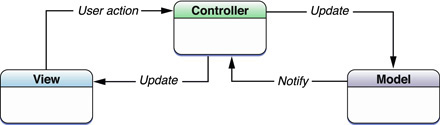
\includegraphics[scale=0.70]{architettura/mvc.png}
\caption{Schema del pattern MVC}
\label{fig:selettore}
\end{figure}

Nei prossimi paragrafi verranno descritte le classi principali del progetto.

\section{Diagramma delle classi}
\chapter{Dettagli implementativi rilevanti}
\chapter{Sviluppi futuri}

%  \chapter{Style features of \textsf{sapthesis}}
% 
% In this chapter I will discuss my stylistic choices of \textsf{sapthesis}.
% I will show the page layout geometry and I will describe the page style.
% 
% \section{Page layout}
% 
% The page is fixed at the dimensions of an A4 paper, therefore you have to print your thesis on A4 paper to obtain the best results. The font dimension is fixed at 11\, pt. The text column and the margins are chosen to fill to the best an A4 paper while keeping a reasonable line length (396\, pt) for a good readability. The text height and the text width are in golden ratio (\textasciitilde 1.6180) as well as the outer and inner margins in a two-side document after binding margin removal. Also the top margin (excluding the header) and bottom margin are in the golden ratio. In Fig.~\ref{layout} a sketch of the \textsf{sapthesis} page layout is shown.

% \begin{figure}[h]
% \centering
% \setlength{\unitlength}{0.27mm}
% \begin{picture}(420,297)(-210,0)
% \polyline(-210,0)(210,0)(210,297)(-210,297)(-210,0)
% \Line(0,0)(0,297)
% \put(27.05,37.4){\polygon(0,0)(139.2,0)(139.2,223.8)(0,223.8)}
% \put(-27.05,37.4){\polygon(0,0)(-139.2,0)(-139.2,223.8)(0,223.8)}
% \put(27.05,268.16){\polygon(0,0)(139.2,0)(139.2,4.22)(0,4.22)}
% \put(-27.05,268.16){\polygon(0,0)(-139.2,0)(-139.2,4.22)(0,4.22)}
% \end{picture}
% \caption{Page layout scheme of \textsf{sapthesis class} using a zero binding margin.}
% \label{layout}
% \end{figure}


% \section{Page style}
% 
% The captions have a smaller font respect to the text and the label is in boldface. The appearance of the margin notes has been improved.
% They have the same font dimension of the footnotes and are typed in italics.
% Moreover I defined a new command to typeset margin note aligned to the left on the right page and vice versa on the left page.
% Notice that if a binding margin greater than 1.5\, cm is used, the dimensions of the margin notes become too small and very ugly.
% Do not use them in this case.
% 
% The mathematical objects, figures and tables are numbered within the chapters (e.g. 1.1, 1.2,\ldots for the first chapter, 2.1, 2.2 for the second one and so on\ldots). See for example the number of this simple equation
% \begin{equation}
% x_{1,2}=\frac{-b\pm\sqrt{b^2-4ac}}{2a}
% \end{equation}
% 
% 
% The title page is automatically composed when the \texttt{\bs maketitle} command is given.
% The parameters needed for the title page, author, title, etc\ldots , are supplied by dedicated commands explained in the next section.
% Two copies of the university logo in \texttt{pdf} format, one for color printing and the other one for black and white printing, are supplied in the \textsf{sapthesis} package. They are shown in Fig.~\ref{fig:largenenough}.
% 
% \begin{figure}
% \centering
% 
\includegraphics[width=0.7\textwidth]{sapienza-MLred-pos}\\[3ex]
% 
\includegraphics[width=0.7\textwidth]{sapienza-MLblack-pos}
% \caption{Logo of the Sapienza -- University of Rome.}
% \label{fig:largenenough}
% \end{figure}
% 
% 
% 
% \section{About figures and tables}
% 
% As regards the image formats, please use vector images as much as possible! Use jpg images only for photographs! pdf\LaTeX\ supports the pdf, jpg and png formats.
% 
% A very simple table is show in Tab.~\ref{tab:letters}. Remember to typeset
% always the table caption above the table. Do not use vertical lines.
% 
% \begin{table}
% \caption{This is a simple table.}
% \label{tab:letters}
% \centering
% \begin{tabular}{lcc}
% \toprule
% Letter & Test & Test \\
% \midrule
% A & C & E \\
% B & D & F \\
% \bottomrule
% \end{tabular}
% \end{table}
% 
% 
% \section{A section}
% 
% In this manual you can skip the gray text because it is just dummy text.
% 
% \textcolor{gray}{\lipsum[1-10]}
% 
% 
% 
% \section{Another section}
% 
% In this manual you can skip the gray text because it is just dummy text.
% 
% \textcolor{gray}{\lipsum}
% 
% 
% \appendix
% \chapter{Special commands provided by \textsf{sapthesis}}
% 
% \textsf{Sapthesis} provides some special commands, particularly useful for scientific works. You can use for example the roman shape, instead of the italic, for the imaginary unit (\texttt{\bs iu}) and Napier's number (\texttt{\bs eu}):
% \begin{equation}
% \eu^{\iu\pi}+1=0
% \end{equation}
% 
% There are also two commands to speed up the writing of derivatives. In the following example we have used the commands \texttt{\bs der} and \texttt{\bs pder}):
% \begin{equation}
% \der{f}{x} \qquad \pder[2]{f}{y}
% \end{equation}
% 
% 
% \textsf{Sapthesis} provides also 4 commands to improve the writing of subscripts, \texttt{\bs rb} and \texttt{\bs tb}, and superscripts, \texttt{\bs rp} and \texttt{\bs tp}. Two of these commands, \texttt{\bs rb} and \texttt{\bs rp}, can be used both in text and in math mode and compose their argument in roman. The other two, \texttt{\bs tb} and \texttt{\bs tp}, can be used only in text mode and compose their argument as are. Here it is an usage example of \texttt{\bs rb} and \texttt{\bs rp}:
% \[
% a_b \neq a\rb{b}\qquad a^b \neq a\rp{b}
% \]
% And here it is an usage example of \texttt{\bs tb}: \emph{Cu\tb{It} indicates copper bought in Italy}. And a usage example of \texttt{\bs ts}: \emph{Cher G\tp{le} Napol\'eon}.
% 
% 
% Then several commands for the correct typesetting of unit of measurements are provided. For example the command \texttt{\bs un} typesets its argument in roman and leaves a thin space between the number and the unit: $25\un{m}$, $3.5\un{m/s}$. Other commands are: (\texttt{\bs g}) 45\g, (\texttt{\bs C}) 30\,\C, (\texttt{\bs A}) 12\,\A, (\texttt{\bs micro}) 40\,\micro m, (\texttt{\bs ohm}) 27\,\ohm. 
% 
% We have also \texttt{\bs x} as abbreviation of \texttt{\bs times}: \$7 \bs x 10\^{}5\$ gives $7 \x 10^5$. Then \texttt{\bs di} is the differential symbol which automatically insert the correct spacing.
% \[
% \int x \di x
% \]
% 
% Finally we have defined the color \textsf{sapred} which is the official color
% of Sapienza -- University of Rome. It is defined as RGB(130,36,51). \textcolor{sapred}{This text is written with the color \textsf{sapred}.}
% 
% In the following dummy text you can observe the usage of \texttt{\bs mnote} command which typesets fancy margin notes.
% 
% \textcolor{gray}{\lipsum}
% \marginpar{This is a fancy margin note!}
% \textcolor{gray}{\lipsum}

\backmatter
% bibliography
%\cleardoublepage
%\phantomsection
%\bibliographystyle{sapthesis} % BibTeX style
%\bibliography{bibliography} % BibTeX database without .bib extension

\end{document}
